\chapter{Prodotti software}\label{ch-01}

\lecturemeta{Capitolo originale: 1 --- Software products \quad\textbullet\quad Antonio Brogi}{Appunti di Emiliano Sescu (github.com/Faxatos), cap. 1}

\section{Software engineering
project-based}\label{software-engineering-project-based}

L'ingegneria del software \textbf{project-based} (orientata al progetto)
è la forma più antica di ingegneria del software. Si parte da una
richiesta del cliente e, alla fine del progetto, si consegna al cliente
il software richiesto.

Il problema principale è che il cliente deve scrivere i
\textbf{requisiti} (cioè la descrizione di cosa il software deve fare)
in un formato preciso, parlando di cose che di solito non conosce: il
cliente non ragiona in termini di requisiti software, ma è costretto a
produrli. In più i requisiti \textbf{non sono fissi}: cambiano a ogni
incontro, perché il cliente capisce via via cosa il software può fare
per lui.

\begin{figure}[H]
\centering
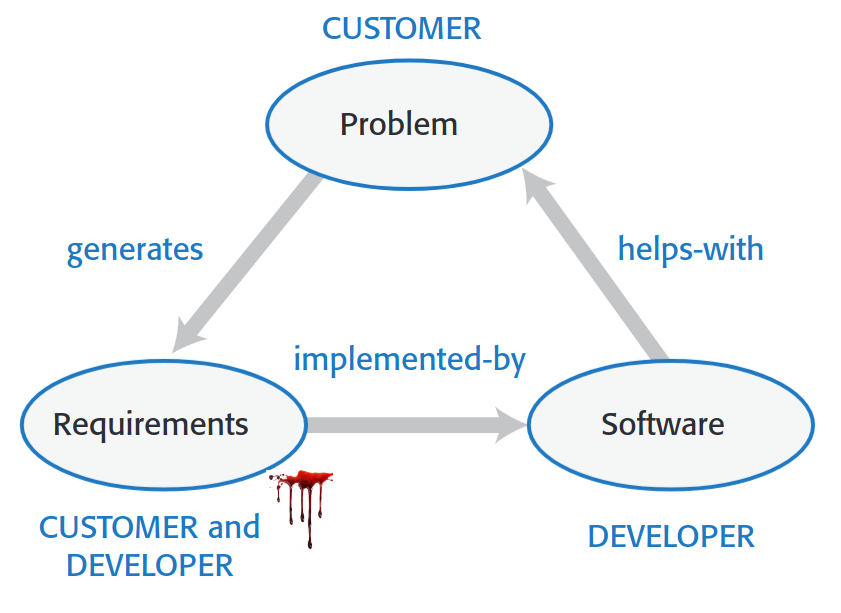
\includegraphics[width=0.60\linewidth,height=0.45\textheight,keepaspectratio]{images/01-prodotti_fig1-1_ciclo-project-based.png}
\caption{Ciclo di vita del software project-based.}
\end{figure}

Con il tempo gli sviluppatori tendono a passare da tanti prodotti fatti
su misura per clienti diversi a \textbf{un unico prodotto} che vada bene
per tutti.

\begin{boxtip}{Software generico}

Per la maggior parte delle aziende gli utenti non hanno bisogno di
software su misura, ma di \textbf{software generico} che risolva
problemi comuni.

\end{boxtip}

\section{Software engineering
product-based}\label{software-engineering-product-based}

Nell'ingegneria del software \textbf{product-based} (orientata al
prodotto) è il team di sviluppo a decidere quali sono le funzionalità
(\emph{feature}) del software e come cambierà nel tempo. Il cliente esce
dal ciclo: sono gli sviluppatori a scegliere cosa costruire, e quindi
devono individuare le feature che rispondono ai bisogni dei clienti.

\begin{figure}[H]
\centering
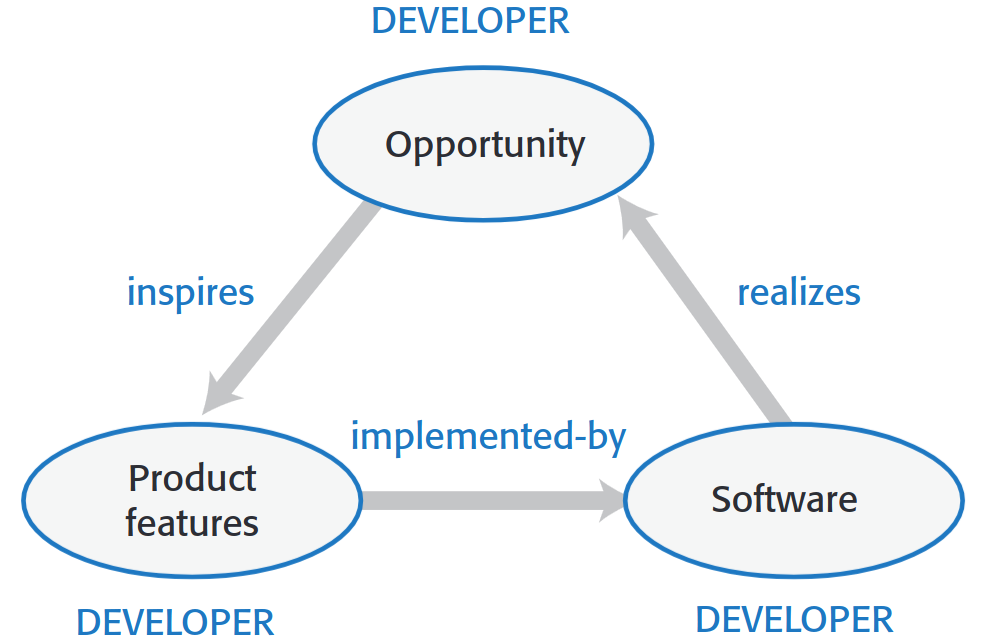
\includegraphics[width=0.60\linewidth,height=0.45\textheight,keepaspectratio]{images/01-prodotti_fig1-2_ciclo-product-based.png}
\caption{Ciclo di vita del software product-based.}
\end{figure}

Un requisito tipico dei prodotti è la \textbf{velocità}: bisogna
sviluppare in fretta, altrimenti qualcun altro occupa quella fetta di
mercato. Il tempo è critico, ed è per questo che si usano i
\textbf{metodi agili}.

\subsection{Modelli di esecuzione}\label{modelli-di-esecuzione}

Esistono tre modi in cui un prodotto software può essere eseguito:

\begin{itemize}
\tightlist
\item
  \textbf{Stand-alone}: interfaccia utente, funzionalità e dati stanno
  tutti sul computer dell'utente. Il fornitore (\emph{vendor}) si occupa
  solo di creare e inviare gli aggiornamenti.
\item
  \textbf{Ibrida} (\emph{hybrid}): una parte dell'applicazione è sul
  dispositivo dell'utente (interfaccia, dati utente, aggiornamenti) e
  una parte sul server del fornitore (logica di business e backup dei
  dati).
\item
  \textbf{Software as a Service (SaaS)}: l'utente non installa nulla, ha
  solo un'interfaccia (browser o app). Il programma gira sul server del
  fornitore, quindi è più facile gestirlo e aggiornarlo senza doverlo
  distribuire.
\end{itemize}

\begin{figure}[H]
\centering
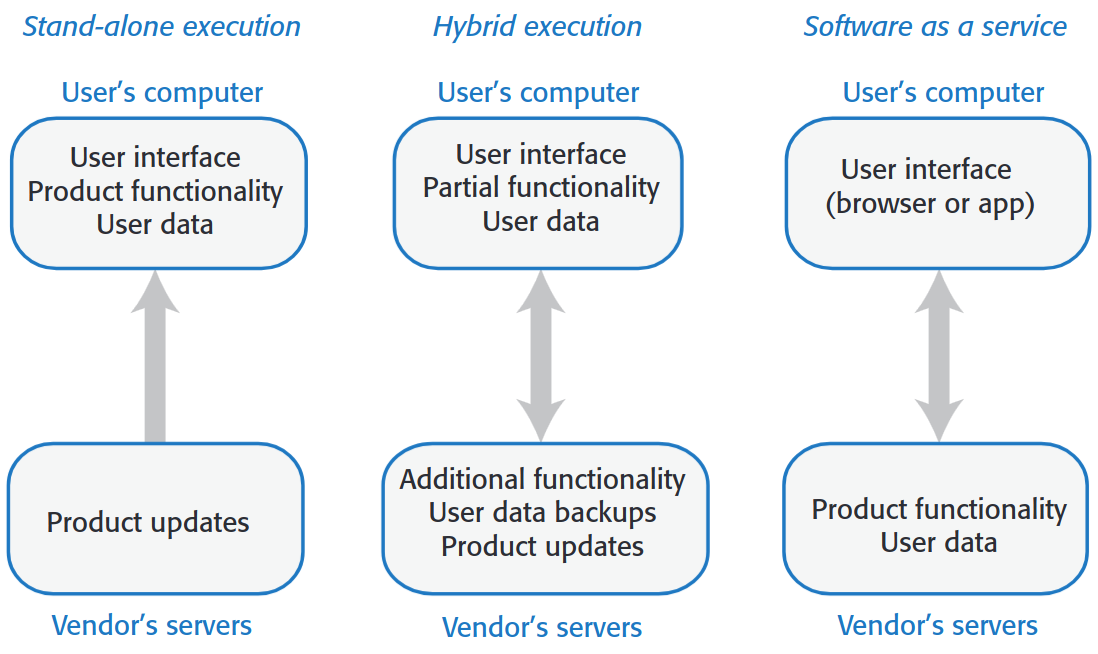
\includegraphics[width=0.66\linewidth,height=0.45\textheight,keepaspectratio]{images/01-prodotti_fig1-3_modelli-esecuzione.png}
\caption{Modelli di esecuzione.}
\end{figure}

\section{Product vision}\label{product-vision}

Ogni nuovo prodotto software dovrebbe avere una \textbf{visione}
(\emph{product vision}) che risponde a tre domande: \textbf{chi} sono i
clienti a cui ci rivolgiamo? \textbf{Cosa} stiamo sviluppando?
\textbf{Perché} i clienti dovrebbero comprarlo?

Per gli sviluppatori è comodo riassumere la visione in una scheda con
questa struttura:

\begin{boxdefinition}{Schema della product vision}

\textbf{FOR} (cliente target) \textbf{WHO} (bisogno o opportunità)

\textbf{THE} (nome del prodotto) \textbf{is a} (categoria del prodotto)
\textbf{THAT} (beneficio chiave, motivo per comprarlo)

\textbf{UNLIKE} (principale alternativa concorrente) \textbf{OUR
PRODUCT} (cosa ci distingue dai concorrenti)

\end{boxdefinition}

\begin{boxexample}{Il sistema iLearn (dal libro di Sommerville)}

\textbf{Per} insegnanti ed educatori \textbf{che} hanno bisogno di
aiutare gli studenti a usare risorse didattiche online, \textbf{iLearn}
è un ambiente di apprendimento aperto \textbf{che} permette agli
insegnanti stessi di configurare facilmente le risorse per le loro
classi. \textbf{A differenza} degli ambienti come Moodle, centrati sulla
gestione di materiali e valutazioni, \textbf{il nostro prodotto} mette
al centro il processo di apprendimento.

\end{boxexample}

Le fonti da cui nasce una buona visione sono:

\begin{itemize}
\tightlist
\item
  \textbf{Esperienza nel dominio} (\emph{domain experience}): chi
  sviluppa lavora già in un certo settore (es. marketing e vendite),
  conosce il software che serve e ne vede i difetti, quindi intravede
  spazio per un sistema migliore.
\item
  \textbf{Esperienza sul prodotto} (\emph{product experience}): chi usa
  software esistente (es. un word processor) può trovare modi più
  semplici per offrire le stesse funzionalità. I nuovi prodotti possono
  anche sfruttare tecnologie recenti (es. interfacce vocali).
\item
  \textbf{Esperienza con i clienti} (\emph{customer experience}):
  parlando a lungo con i potenziali clienti si capiscono i loro problemi
  e i vincoli che li limitano (es. l'interoperabilità con altri
  sistemi), oltre alle caratteristiche per loro irrinunciabili.
\item
  \textbf{Prototipazione e sperimentazione}: se l'idea c'è ma non è
  ancora chiara, un prototipo permette di esplorarla e di raccogliere
  feedback dai clienti (che ragionano in termini di funzionalità). Il
  feedback guida il prototipo successivo.
\end{itemize}

\section{Software product management}\label{software-product-management}

Il \textbf{Product Manager} (PM) deve assicurarsi che il team implementi
feature che portano \textbf{valore reale} ai clienti. Per farlo deve
bilanciare tre forze (vedremo che alcune tecniche Agile lo aiutano):

\begin{itemize}
\tightlist
\item
  \textbf{Bisogni di business}: tutto lo sviluppo va gestito tenendo
  conto degli obiettivi sia del cliente sia dell'azienda.
\item
  \textbf{Esperienza dei clienti}: raccogliere regolarmente il feedback
  dei clienti su come usano il prodotto.
\item
  \textbf{Vincoli tecnologici}: tenere conto dei limiti tecnologici
  dell'azienda e dell'hardware/tecnologia che il cliente già usa.
\end{itemize}

\begin{figure}[H]
\centering
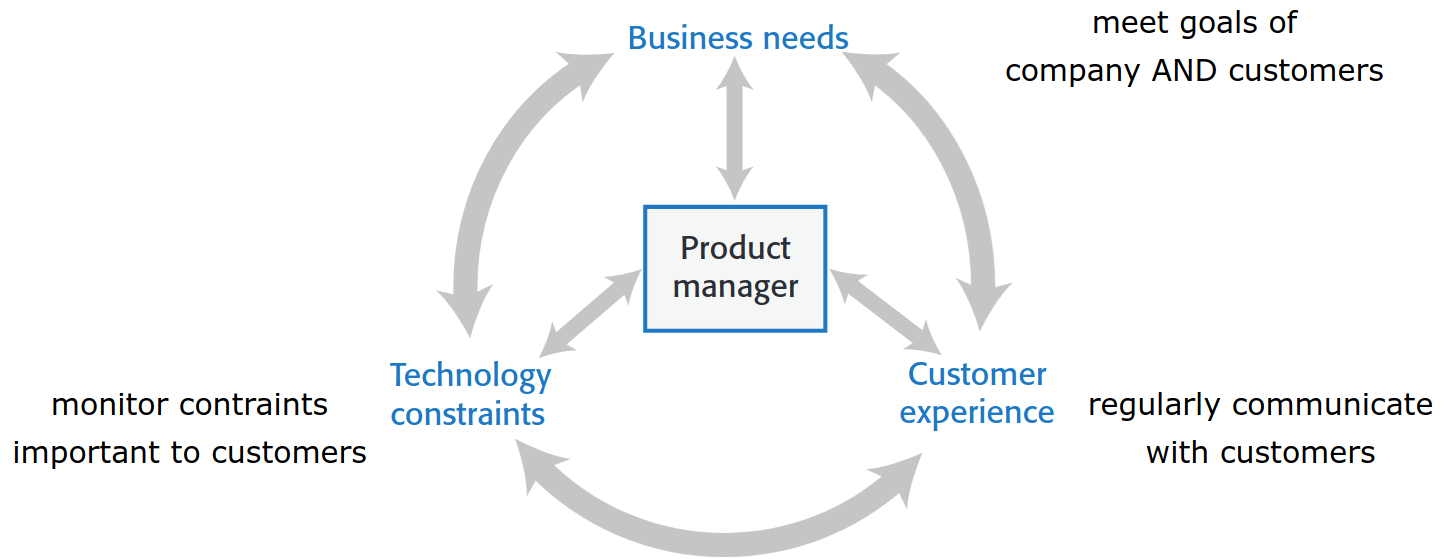
\includegraphics[width=0.73\linewidth,height=0.45\textheight,keepaspectratio]{images/01-prodotti_fig1-4_product-manager.png}
\caption{Compiti del Product Manager.}
\end{figure}

Sul piano tecnico il PM si occupa di:

\begin{itemize}
\tightlist
\item
  \textbf{Product roadmap}: obiettivi, milestone, criteri di successo e
  strade alternative se gli obiettivi non vengono raggiunti.
\item
  \textbf{User story e scenari}, per individuare le feature del
  prodotto.
\item
  \textbf{Product backlog}: la lista delle cose da fare per completare
  lo sviluppo.
\item
  \textbf{Acceptance testing}: test usati lungo tutto il ciclo di vita
  per verificare che ogni release raggiunga gli obiettivi fissati.
\item
  \textbf{Customer testing}: raccolta di feedback su usabilità e
  feature.
\item
  \textbf{UI design}, per avere un'interfaccia semplice e naturale.
\end{itemize}
